\documentclass[Report]{IEEEtran}
\usepackage{xcolor}
\usepackage{cite}
\usepackage{amsmath,amssymb,amsfonts}
\usepackage{algorithmic}
\usepackage{graphicx}
\usepackage{textcomp}
\usepackage{xcolor}

\def\BibTeX{{\rm B\kern-.05em{\sc i\kern-.025em b}\kern-.08em
    T\kern-.1667em\lower.7ex\hbox{E}\kern-.125emX}}
    
\begin{document}

\title{Evaluating Object Detection For Various Platforms}

\author{
\IEEEauthorblockN{Kyler Martinez,}
\IEEEauthorblockN{Ruben Gutierrez,}
\IEEEauthorblockN{Austin Vinh Tran,}
\IEEEauthorblockN{Nelson Chong,}
\IEEEauthorblockN{\textbf{Mohamed El-Hadedy}}\\
\IEEEauthorblockN{California State Polytechnic University, Pomona}\\
\IEEEauthorblockN{\textit{Department of Electrical and Computer Engineering}}\\
Pomona, California, United States of America
}

\maketitle

\begin{abstract}
Computer vision has become an increasingly important field for products such as self-driving cars and the greater field of electronics. As such, there has been an increase in algorithms to perform object detection of varying capabilities, with a popular being YOLOv5. These algorithms require large amounts of computing and electrical power to support these algorithms. In a desktop environment, this may not be too much of a concern, but problems arise as the computing device decreases in size. If object detection is used in embedded systems or on smaller devices, you must determine if the algorithm can function given the device's power constraints and processor resources [7]. Common microcontrollers cannot execute algorithms like YOLOv5; however, there is an increase in machine learning tasks for microcontrollers due to simplified algorithms for microcontrollers and specialized microcontrollers for machine learning tasks [6]. Despite this, systems can use microcontrollers and devices that can process an algorithm like YOLOv5, but there are additional constraints that bottleneck performance, such as internet speeds. There is no one solution for this problem, and every implementation has flaws, but machine learning on small devices is more accessible as technology develops.
\end{abstract}

\begin{IEEEkeywords}
computer vision, yolov5, raspberry pi, microcontroller, esp32, esp32cam
\end{IEEEkeywords}

\section{Introduction}
YOLO stands for 'You Only Look Once', and is an object detection framework using a single convolutional network. YOLOv5 is the 5th version of the YOLO series that uses Focus structure with CSPdarknet53 as a backbone. It is different from other object detection algorithms because it is a regression-based algorithm that takes in the entire image as a whole as opposed to classification-based algorithms that scans the image one pixel at a time. YOLOv5 classifies images using a grid and predicts where to place bounding boxes based on the established objects, classes, and structures [8]. We tested YOLOv5 on PCs, specifically a desktop and laptop, a Raspberry Pi 4, and used it with an ESP-32 microcontroller. The PCs utilize an x86 processor, which is a CISC architecture. On the other hand, the Pi utilizes an ARM-based CPU, which is RISC architecture, and the ESP32 is a single-core RISCV-based microcontroller, but YOLO did not run on it directly. Various tests are performed to measure and capture the performance metrics. 

\subsection{Metrics}
Performance metrics are important in making trade-offs from the designer's and purchasing perspective. The goal is to understand what factors contribute to the overall system performance, and the importance and costs of these factors [10]. For YOLOv5, there are many factors that affect the overall system, but only the frames per second, inference time, and power consumption are considered in this report. These factors are considered when running the YOLOv5 algorithm on different platforms. The inference time is defined as the time it takes for a forward propagation. The inference time can be computed by dividing FLOPs by FLOPS, where FLOPs is the number of floating point operations and FLOPS is the number of floating point operations per second [9]. Frames per second and inference time have an inverse relationship. A KUMAN Power Meter KW47 [5] was used to measure the power consumption of the Raspberry Pi. For the desktop and laptop, a software called Core Temp [11] was used to monitor the power consumption. The power consumption is calculated by taking the difference between the average power and idle power. The average power is calculated by dividing the sum of the power readings by the number of power readings. The total power of the Pi was considered during its evaluation. From these metrics, trade-offs can be made through performance versus power consumption. For example, the frames per second can be increased by limiting the size of the algorithm but it decreases the performance. These metrics are used to compare how well the algorithm runs on different platforms and can be used to find the most suitable platform for any application. To test the performance metrics, YOLOv5 processes a test set of 31 images and a live camera feed.

\begin{table}[htbp]
\caption{Unit Reference}
\begin{center}
\begin{tabular}{|c|c|}
\hline \textbf{Name}& \textbf{Unit} \\
\hline \textbf{Frames Per Second (FPS)}& \textbf{[frame/s]} \\
\hline \textbf{Inference Time (IT) }& \textbf{[ms]} \\
\hline \textbf{Power}& \textbf{[W]} \\ \hline
\end{tabular}
\label{tab1}
\end{center}
\end{table}

\section{Object Detection on PCs}
When testing YOLOv5 on various devices, it can be inferred that the efficiency of the process is dependent on how strong the CPU is for each machine. For PCs and Laptops, this is especially apparent when compared to smaller devices like the Raspberry Pi. As a result, whenever YOLOv5 is running, the FPS of PCs and laptops is significantly larger. The time to process images and videos from a camera is also significantly shorter. The only drawback is that PCs and Laptops require much more power compared to a Raspberry Pi.

\subsection{Desktop: Intel(R) Core(TM) i7-10700K CPU @ 3.80GHz}

\subsubsection{Testing}
The testing was done through YOLOv5's object detection by processing thirty-three different images of various objects, people, and things. Testing with the camera also works the same way. When the camera is processed with YOLOv5, the detection analyzes every frame of the video. In the case of this test set, the camera recorded for about 12 seconds. In terms of the tabular data, the inference was recorded from the terminal output and FPS can be calculated with the equation 1/Inference. The average power was obtained by recording the power change as YOLOv5 processed each image. This applies to both the image set and the camera set. The average values taken for the calculation of average power increase are only from the time when YOLOv5 processes the images.

\subsubsection{Image Testing}
The results from the image test show that the average FPS of a desktop is approximately 100.1FPS and the average inference is 9.99ms. In comparison to the camera test set, the inference has about a 2ms difference and as a result, the average FPS for the image test set is a little bit lower. The power required to test the images however, is much higher than the camera test set  requiring an average power increase of 31.425W. Fig 1 shows the power increase over time for the image test set.

\begin{table}[]
\centering
\caption{YOLOv5 Results Summary: PC}
\label{}
\begin{tabular}{|l|c|c|}
\hline
\textbf{} & \multicolumn{1}{l|}{\textbf{Process from File}} & \multicolumn{1}{l|}{\textbf{Process from Camera}} \\ \hline
\textbf{Average FPS}   & \textbf{100.1}   & \textbf{125}   \\ \hline
\textbf{Average IT}    & \textbf{9.99} & \textbf{8.0} \\ \hline
\textbf{Average Power} & \textbf{31.425}   & \textbf{12.075}  \\ \hline
\end{tabular}
\end{table}

\begin{figure}[htbp]
\centerline{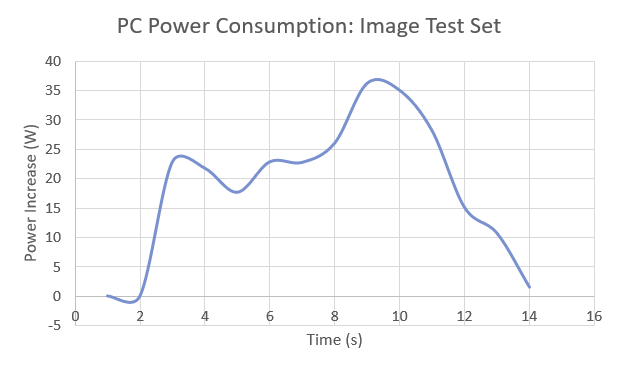
\includegraphics[width=70mm]{PC_Image_Test_Set.png}}
\caption{PC Image Set: Average Power Increase over Time}
\label{fig}
\end{figure}

\subsubsection{Camera Testing}
The results show that the average FPS of a desktop when testing the camera is 125 FPS, which is slightly higher than the image test set. The inference is also consistently around 8.0 which about 2ms faster than the image test set. The most significant difference shown from the tests is the amount of power each test set requires. In the case of the camera, the average power increase was 12.075W which is significantly less power compared to the image test set. Fig 2 shows the power increase over time for the camera test set.

\begin{figure}[htbp]
\centerline{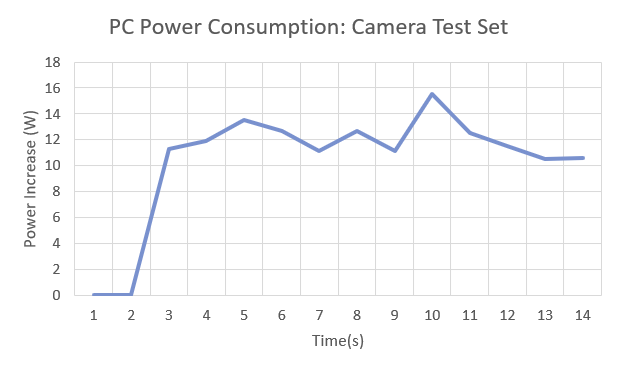
\includegraphics[width=70mm]{PC_Camera_Test_set.png}}
\caption{PC Camera Set: Average Power Increase over Time}
\label{fig}
\end{figure}

\subsection{Laptop: Intel(R) Core(TM) i7-10510U CPU @ 1.80GHz}

\begin{table}[htbt]
\centering
\caption{YOLOv5 Results Summary: Small Weight}
\label{}
\begin{tabular}{|l|c|c|}
\hline
\textbf{} & \multicolumn{1}{l|}{\textbf{Process from File}} & \multicolumn{1}{l|}{\textbf{Process from Camera}} \\ \hline
\textbf{Average FPS}   & \textbf{4.81}   & \textbf{4.11}   \\ \hline
\textbf{Average IT}    & \textbf{208.02} & \textbf{243.18} \\ \hline
\textbf{Average Power} & \textbf{16.3}   & \textbf{14.13}  \\ \hline
\end{tabular}
\end{table}

\subsubsection{Testing}
Testing was done through object detection from images on a file, and a live camera feed. YOLOv5 was tested through different models or weights. The four models are small, medium, large, and extra large. Smaller models are lighter on processing requirements but are less accurate. On the other hand, larger models require more processing power but are more accurate. There is a trade-off between power and performance.

\subsubsection{Process From File}
The results when processing images from a file using the small weight is faster than processing images from a camera, but it draws more power. On average, it draws 16.3W. It takes 208.02ms to process each image and has an average FPS of 4.81.

\begin{figure}[]
\centerline{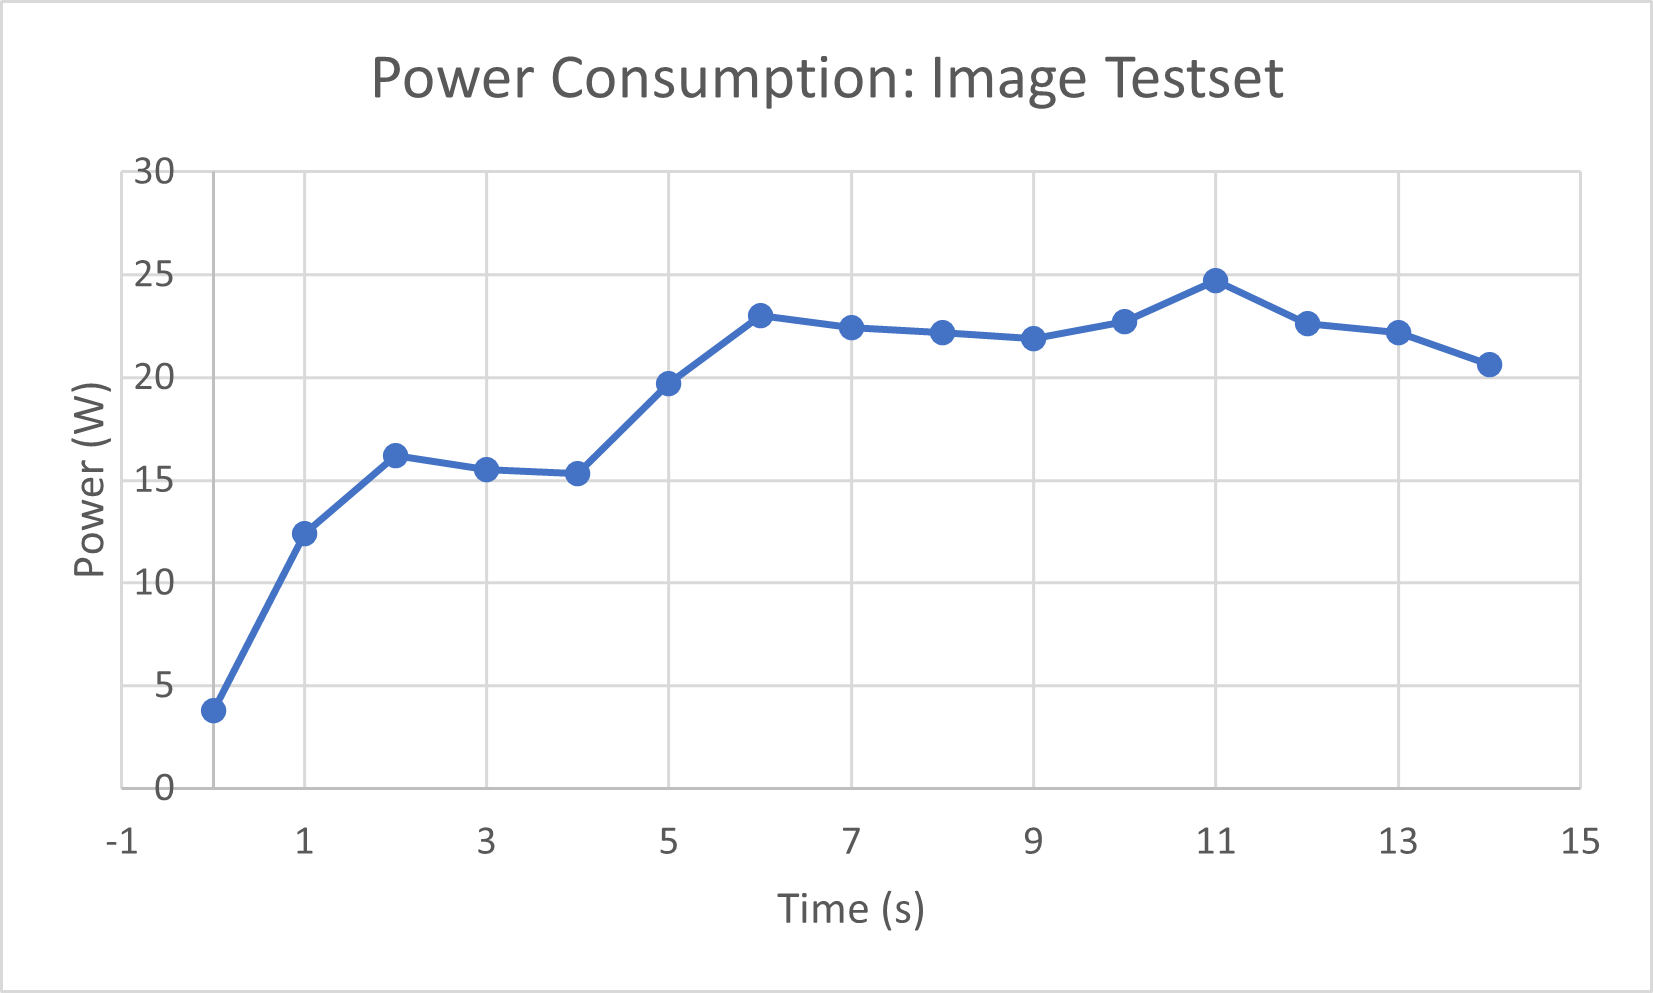
\includegraphics[width=70mm]{Laptop Pictures/Power_File.png}}
\caption{Laptop: Power from Test Images.}
\label{fig}
\end{figure}

\subsubsection{Process From Camera}
The results when processing images through a camera using the small weight is slower than processing images from a file, but it consumes less power. On average, it draws 14.13W and takes 243.18ms to process each image with an average FPS of 4.11. The performance is not much of a difference compared with processing images from a file in terms of FPS and IT but consumes less power, so this is more effective than the first test.

\begin{figure}[htbp]
\centerline{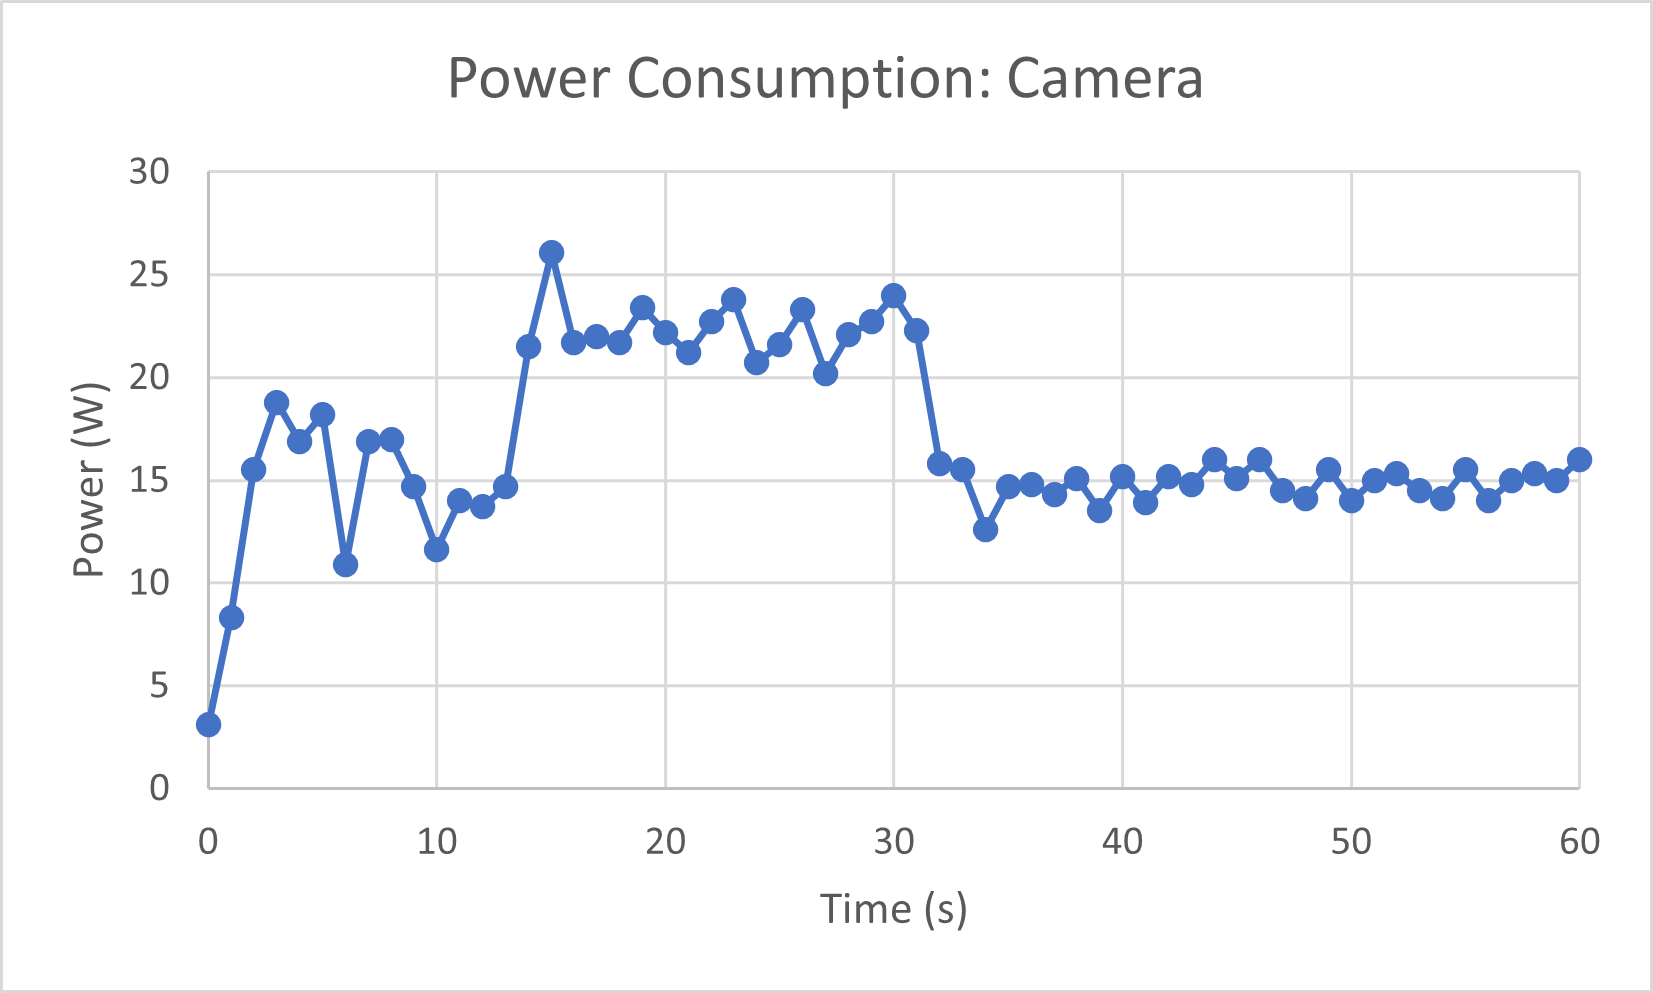
\includegraphics[width=70mm]{Laptop Pictures/Power_Camera.png}}
\caption{Laptop: Power from Camera.}
\label{fig}
\end{figure}


\section{Object Detection on The Raspberry Pi}
The Raspberry Pi is a microprocessor popular for IoT projects due to its small size and relatively low price point. Additionally, the Pi is used to incorporate machine learning on smaller devices with applications in computer vision.

YOLOv5 was tested on the Raspberry Pi to evaluate its performance and the practicality of object detection on small devices like it. Throughout our tests, we used a Raspberry Pi 4 4GB model. In addition to evaluating the algorithm's performance, we tested the effects of cooling and image retrieval methods to evaluate the use cases for the Pi and YOLO.

\subsection{Testing}
For the inference time, we used two general tests with two configurations. The two tests were detection from a file and detection from a USB webcam, and the two configurations were cooling from a 5V fan and no cooling from the fan, which resulted in a total of eight tests.

The file tests used the image dataset and finished in approximately 70 seconds. The camera tests have a duration of 1200 seconds to test the performance after a long period of use. The power test measured the power throughout these tests. For the power test, we the test period is 70 seconds for the camera with cooling and 5 minutes for the camera without cooling.

\subsection{Results}

\begin{table}[htbp]
\caption{Pi 4 YOLOv5 Results Summary}
\begin{center}
\begin{tabular}{|c|c|c|c|c|}
\hline \textbf{ }&\multicolumn{2}{|c|}{\textbf{Process from file}}&\multicolumn{2}{|c|}{\textbf{Process from camera}} \\
\hline \textbf{ }& \textbf{Cooling} & \textbf{No Cooling } & \textbf{Cooling} & \textbf{No Cooling} \\
\hline \textbf{Average FPS}& \textbf{0.65} & \textbf{0.47} & \textbf{0.47} & \textbf{0.33} \\
\hline \textbf{Average IT}& \textbf{1520} & \textbf{2600} & \textbf{2137} & \textbf{2743} \\
\hline \textbf{Average Power}& \textbf{6.0} & \textbf{5.2} & \textbf{7.2} & \textbf{6.7} \\ \hline
\end{tabular}
\label{tab1}
\end{center}
\end{table}

\subsubsection{Results: Process From File}
The Pi performed best when it processed images from disk. When the fan was on, the Pi processed images at an average rate of 0.65 frames per second, while without cooling, it performed at 0.47 frames per second.

When processing images from disk, the Pi draws less power; the cooling test used an average of 6.0W, and the no-cooling test used an average of 5.2W. For both tests, the drawn power was constant during most of the operation.

\begin{figure}[htbp]
\centerline{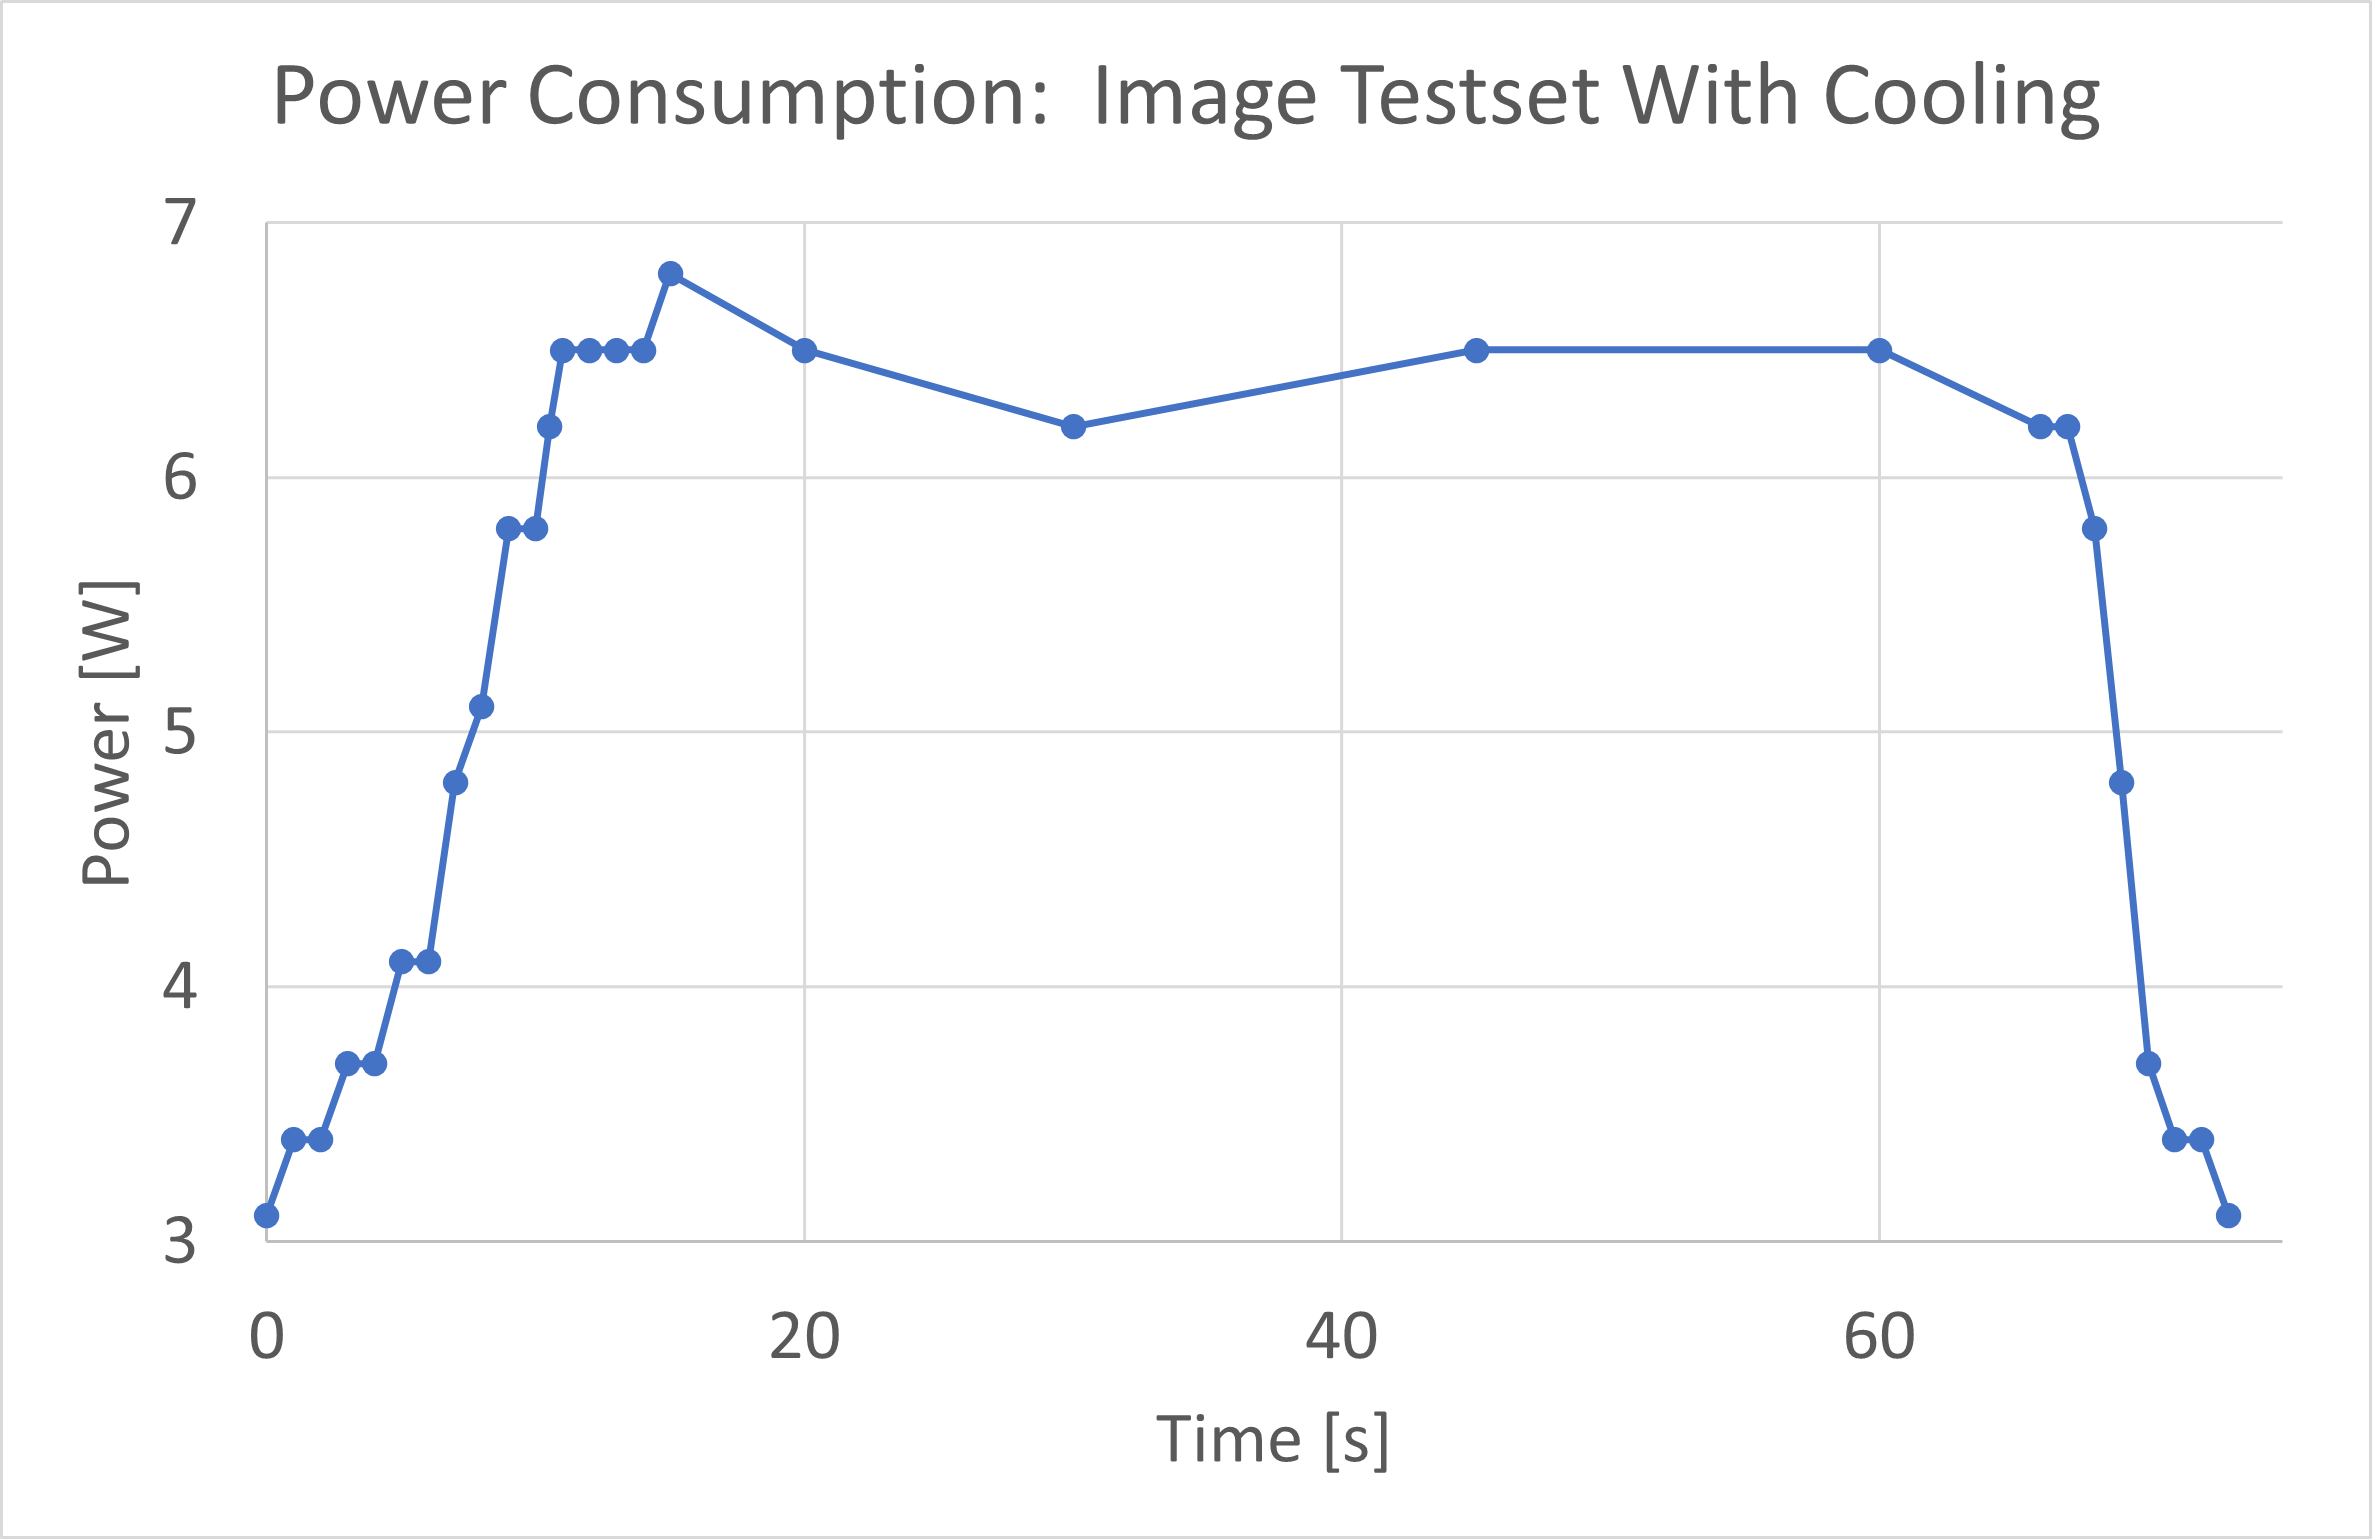
\includegraphics[width=70mm]{Pi_Pictures/Power_I_C.png}}
\caption{Pi 4: Power when cooling is applied.}
\label{fig}
\end{figure}

\begin{figure}[htbp]
\centerline{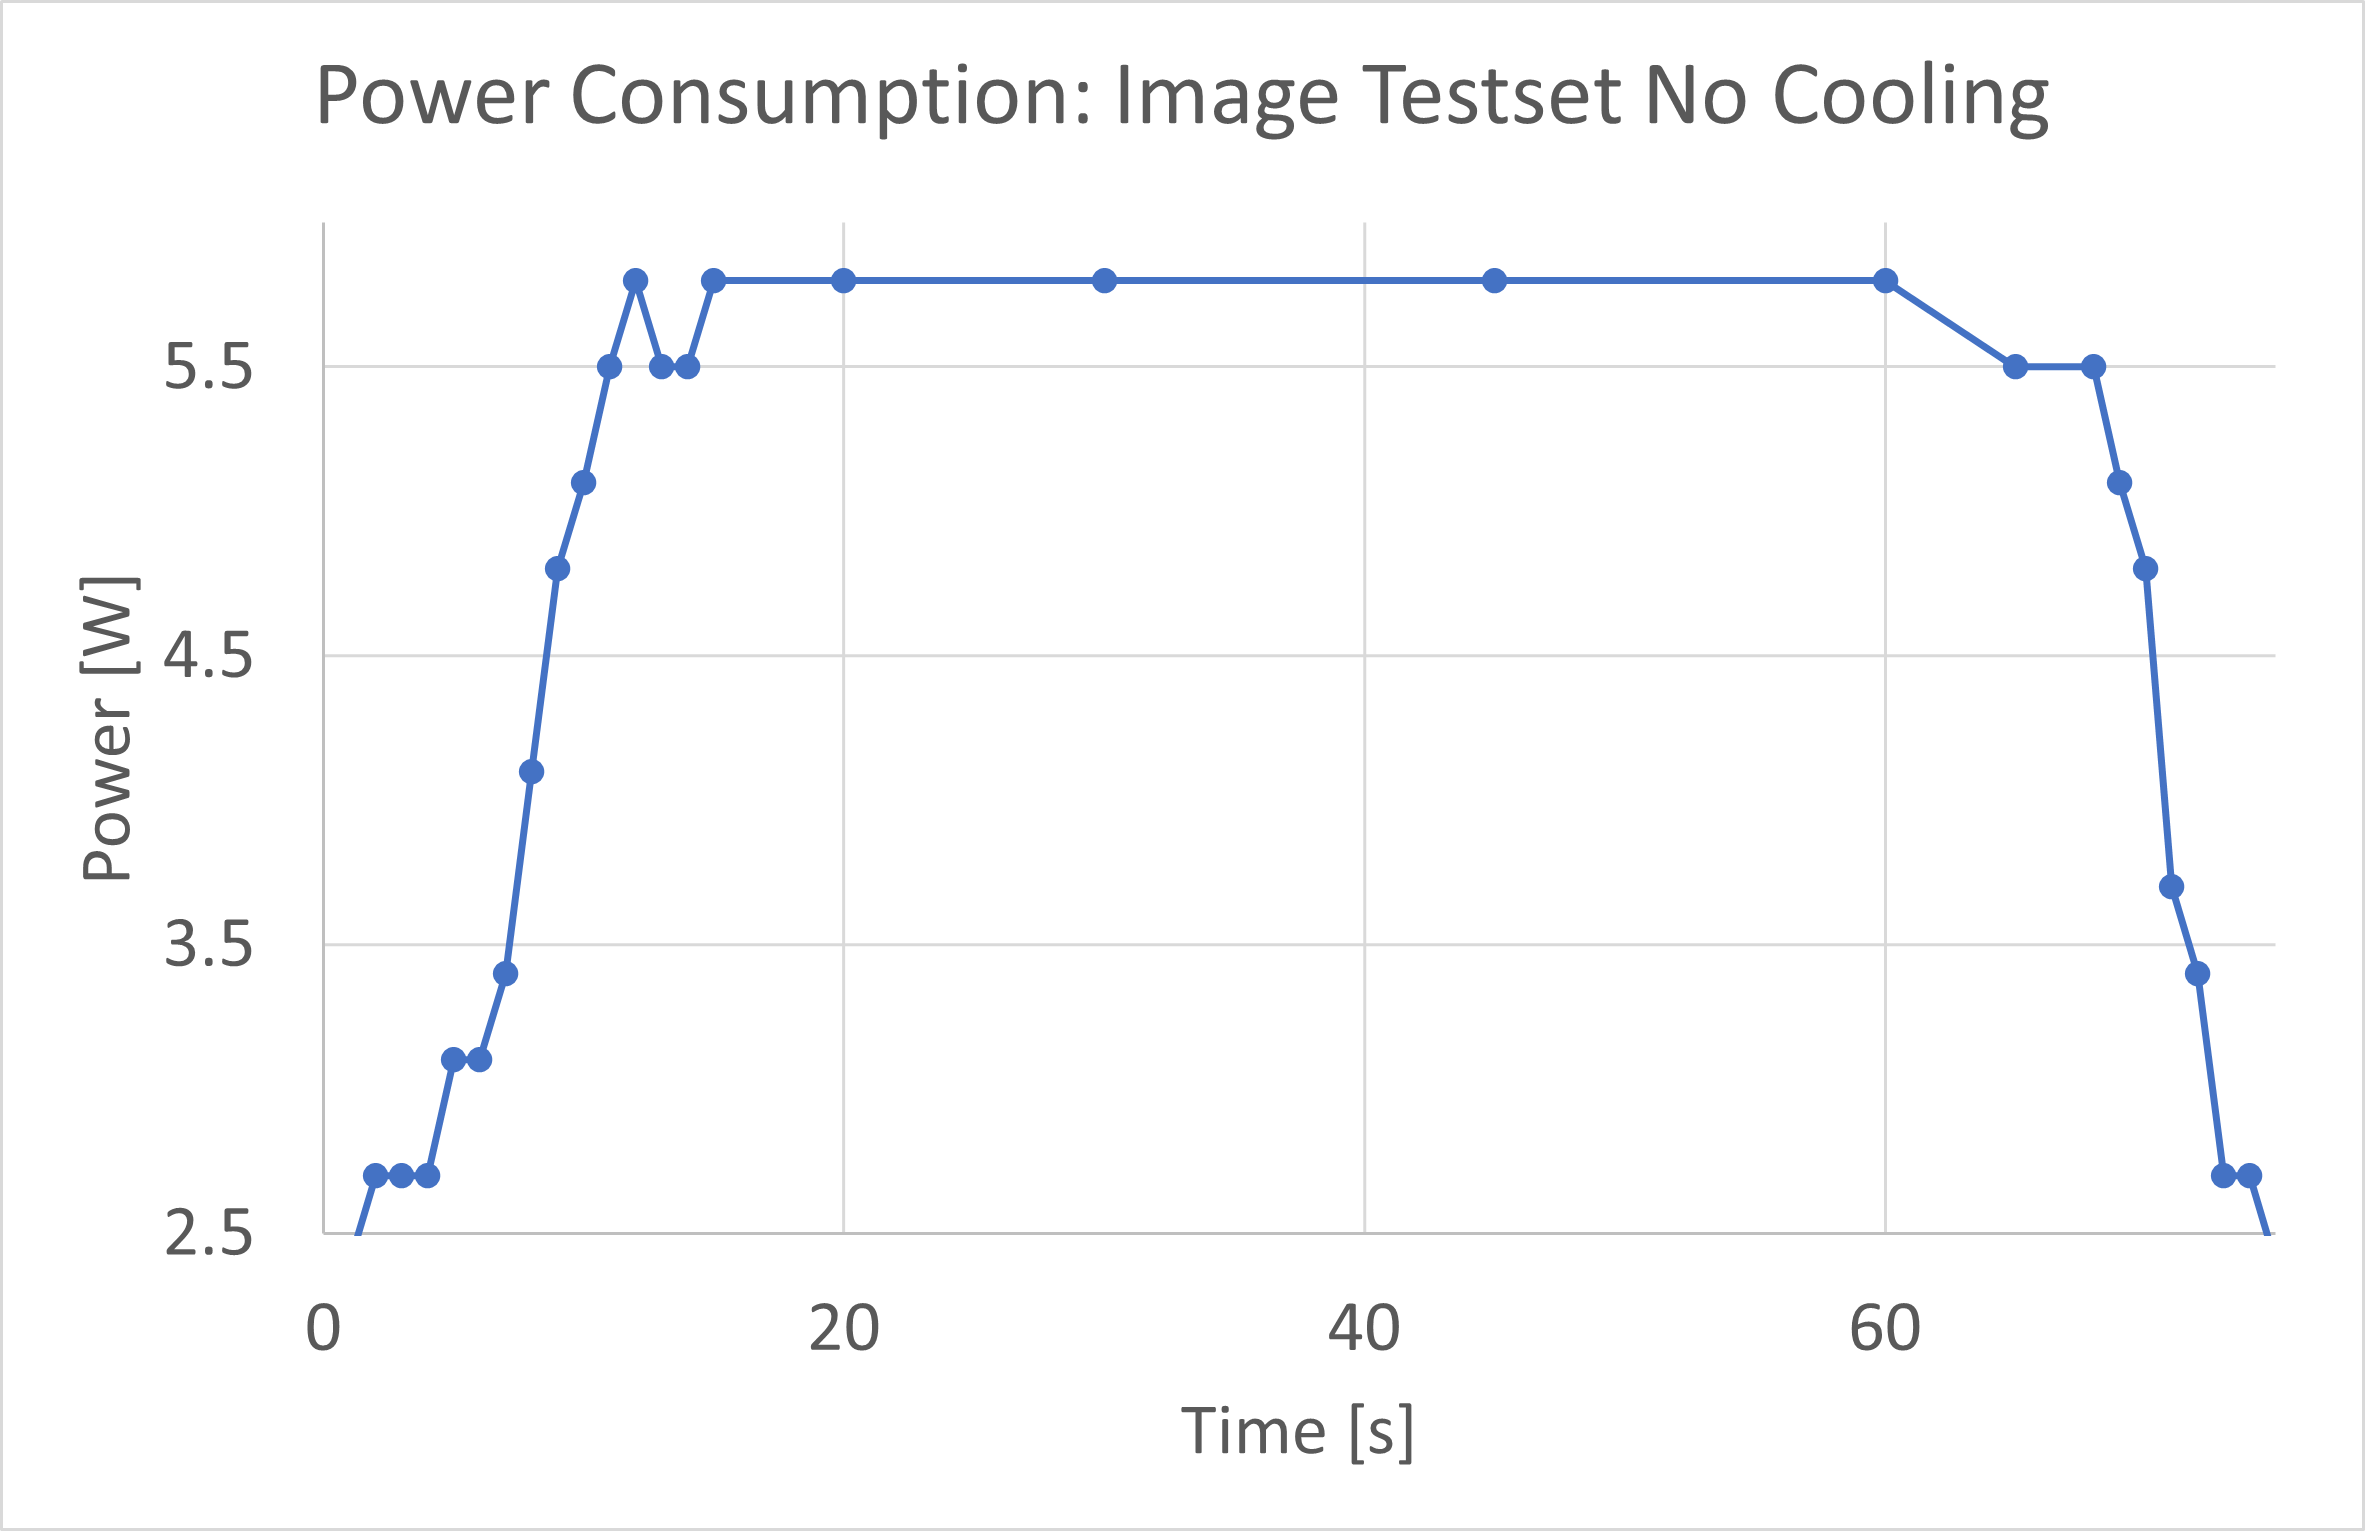
\includegraphics[width=70mm]{Pi_Pictures/Power_I_NC.png}}
\caption{Pi 4: Power when no cooling is applied.}
\label{fig}
\end{figure}

\subsubsection{Results: Process From Camera}
The camera tests performed worse than the image tests with and without cooling. When cooling was applied, the inference time was relatively stable, varying between 2120 and 2180 milliseconds after the first 30 seconds of run time.

\begin{figure}[htbp]
\centerline{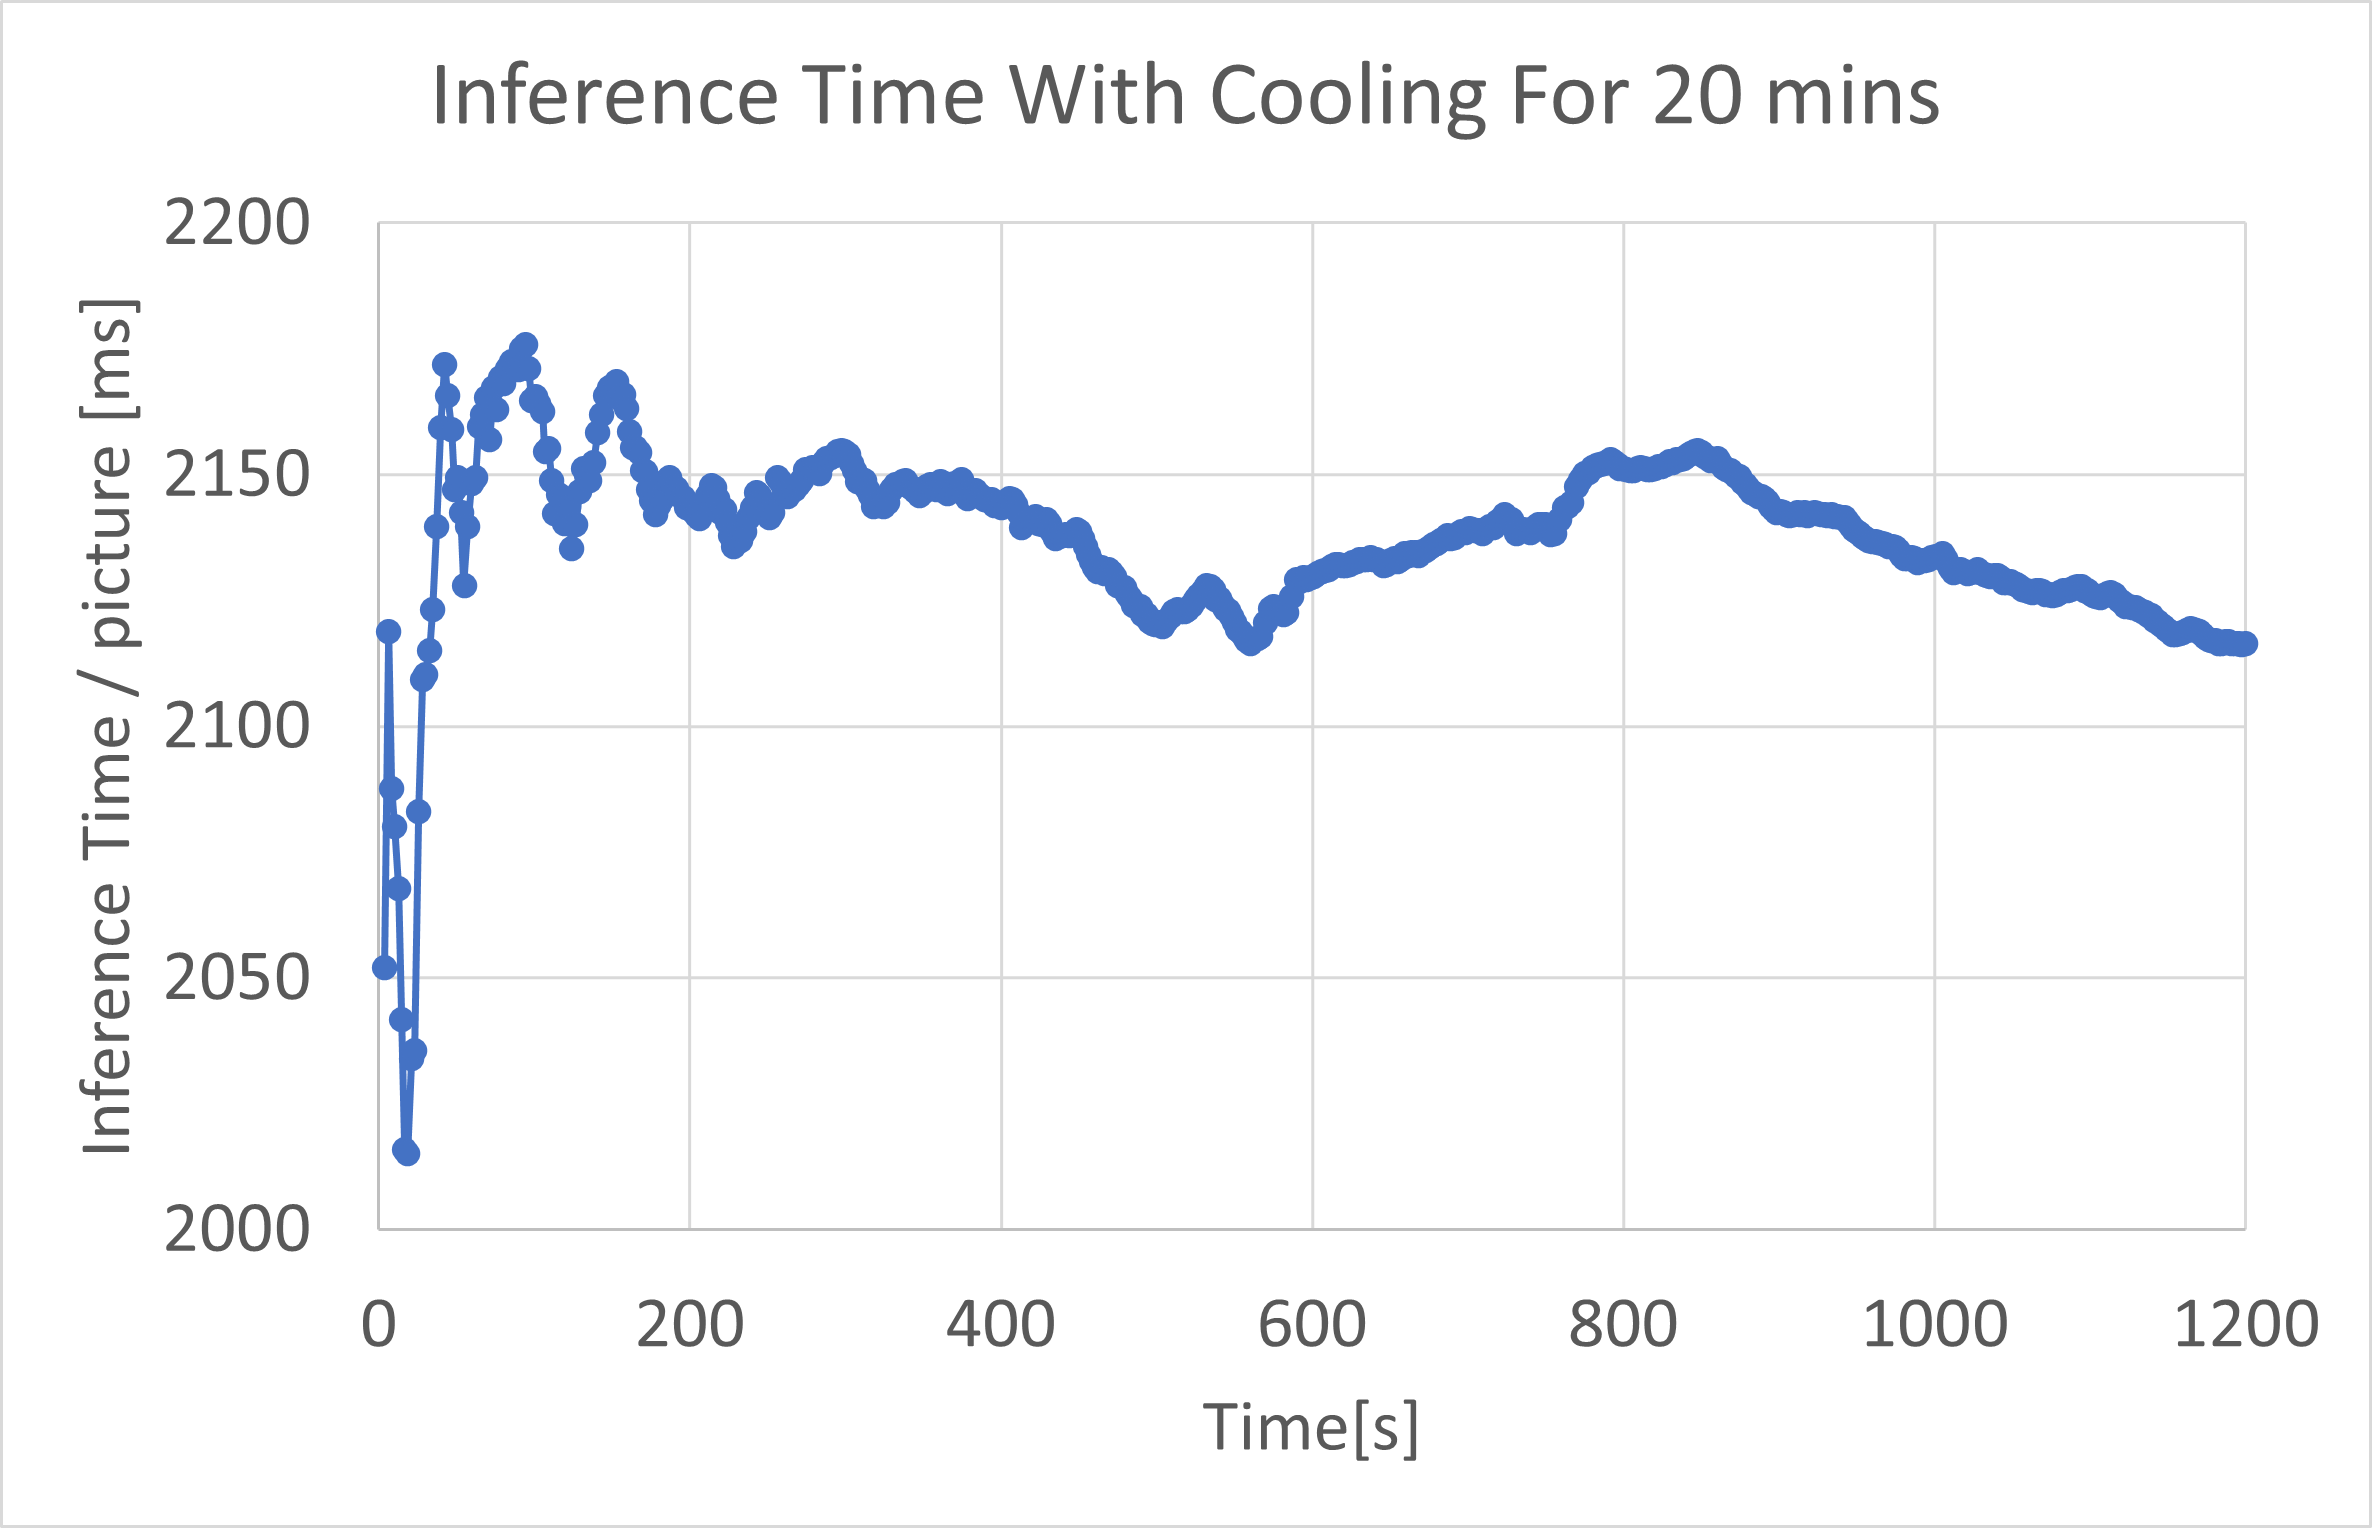
\includegraphics[width=80mm]{Pi_Pictures/Time_C_C.png}}
\caption{Pi 4: Inference time when cooling is applied.}
\label{fig}
\end{figure}

Without cooling, the frame rate did not stabilize to a range of values. The frame rate changed logarithmically, with performance degrading over time. After 20 minutes of use, the inference time was 2985ms per frame, with no signs of stabilizing.

\begin{figure}[htbp]
\centerline{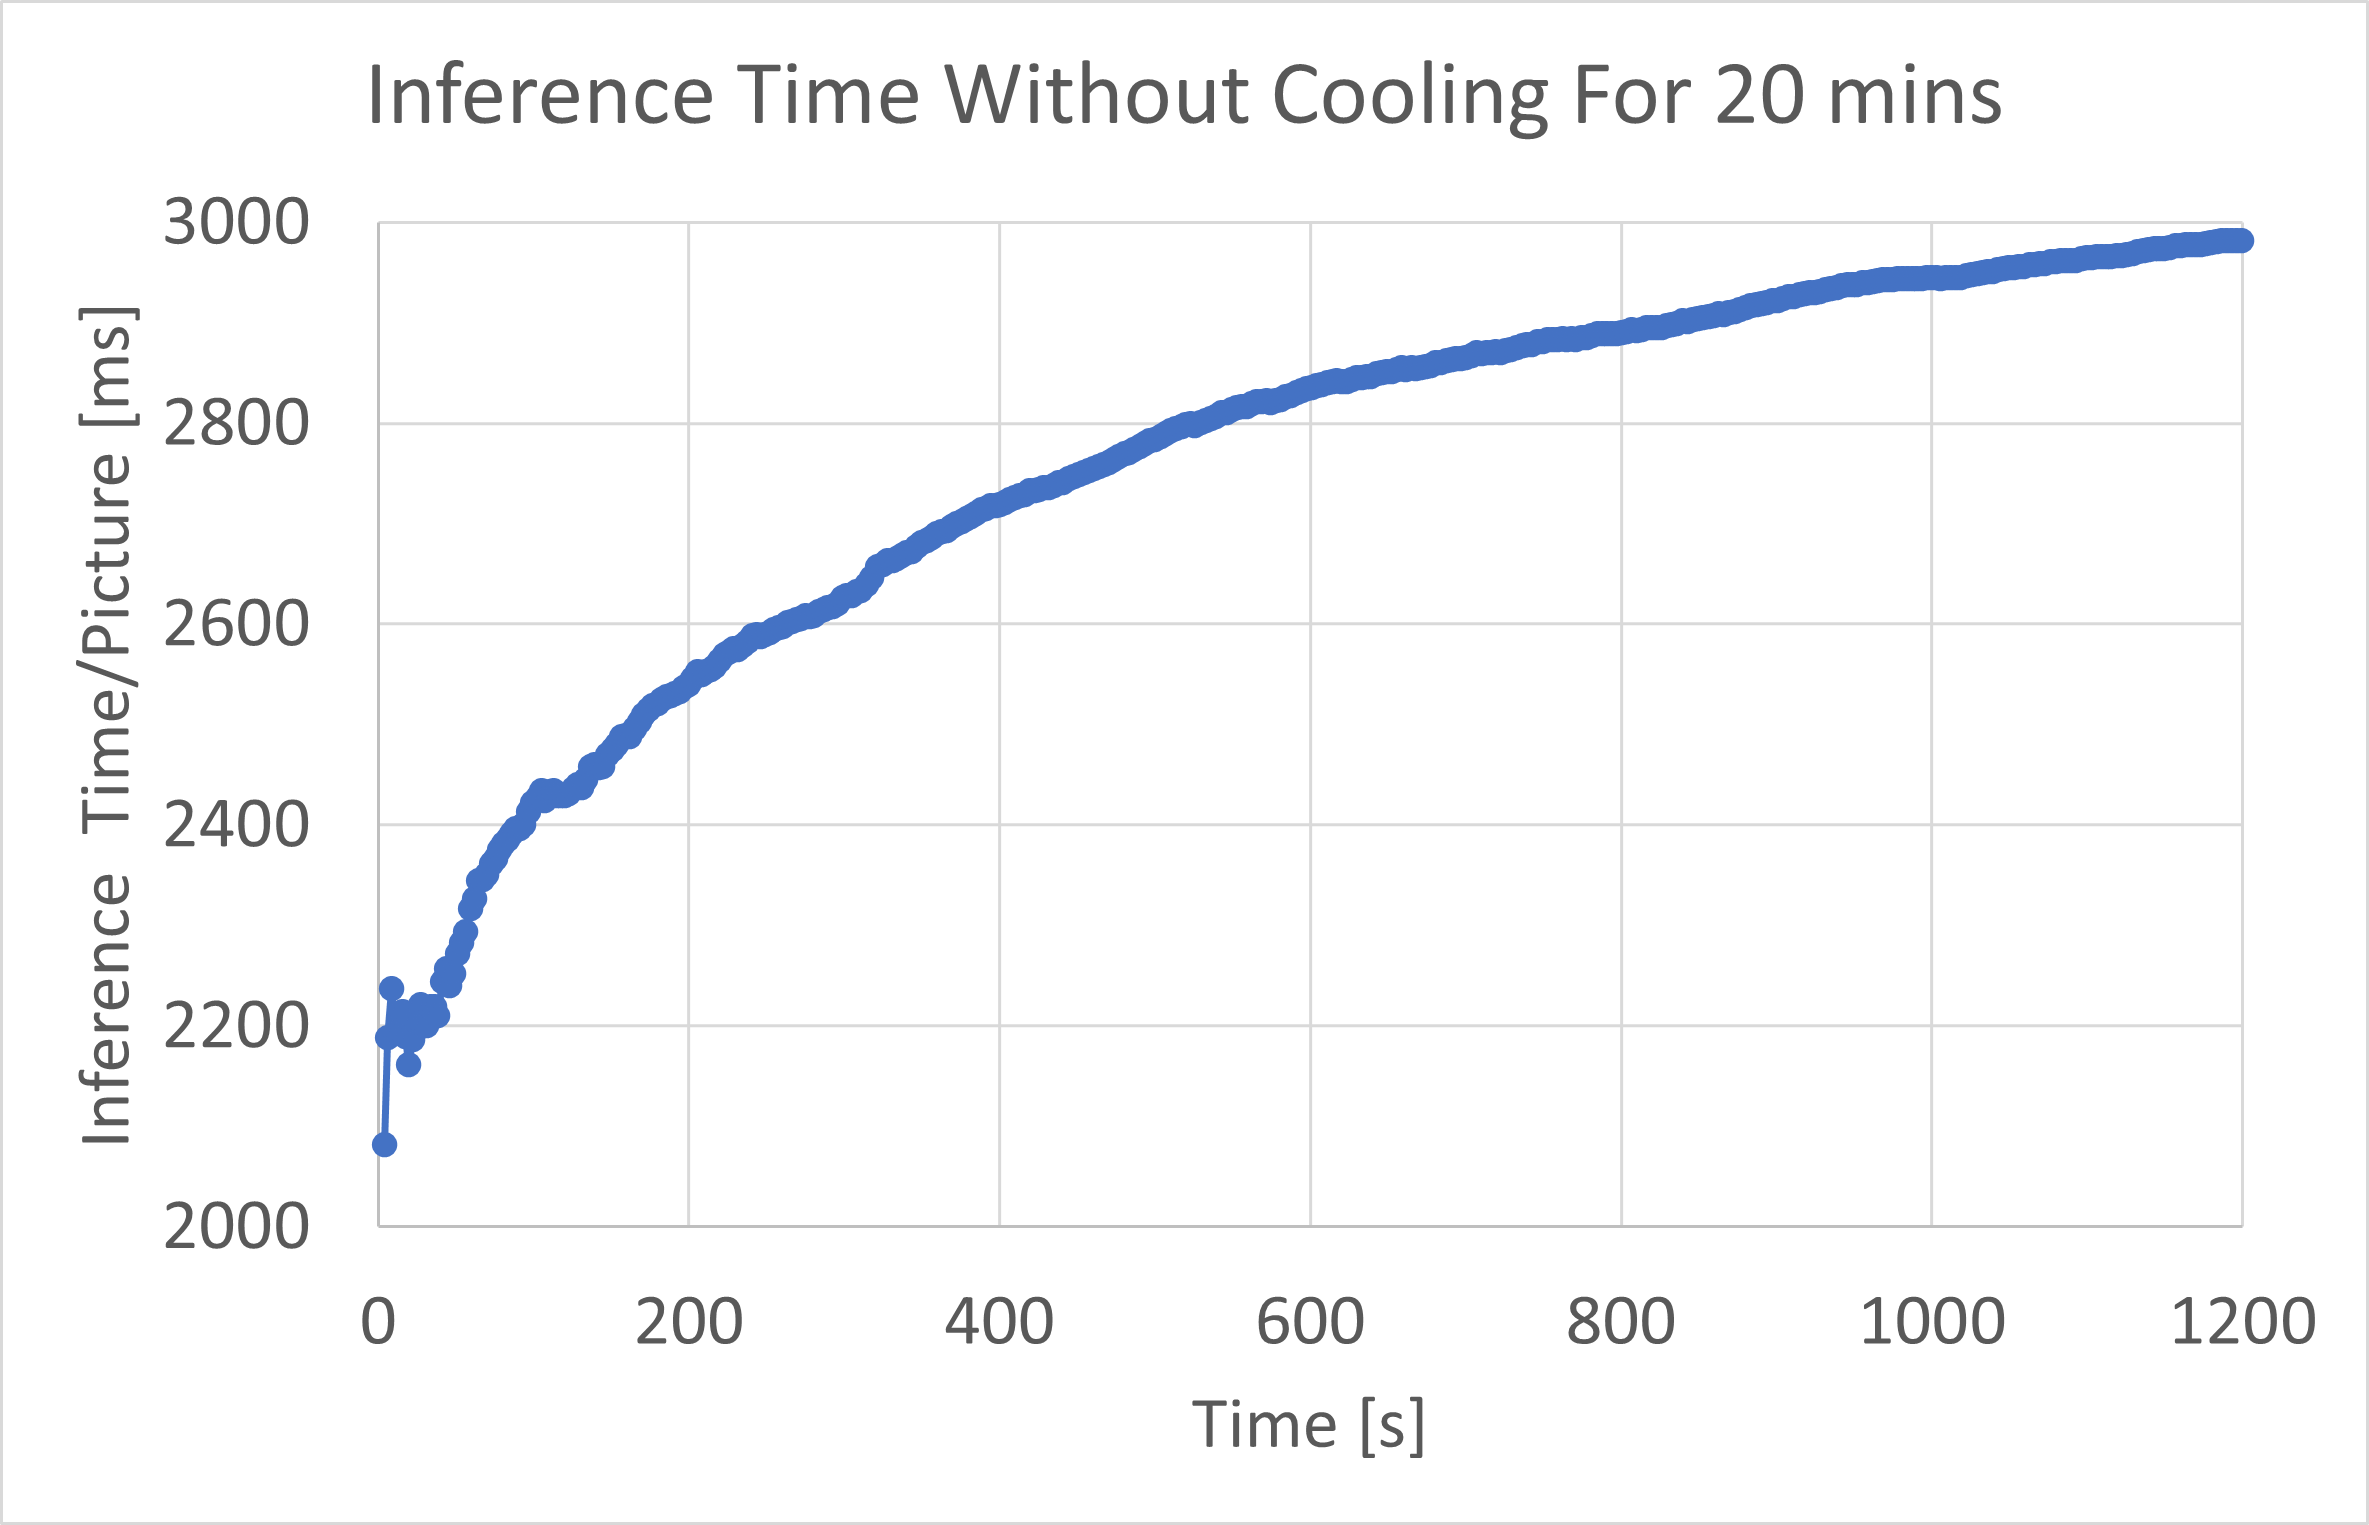
\includegraphics[width=80mm]{Pi_Pictures/Time_C_NC.png}}
\caption{Pi 4: Inference time when no cooling is applied.}
\label{fig}
\end{figure}

The power usage of the Pi reflects behavior similar to the inference time. For the cooling test, the power drawn was consistent for most of the test's duration. The power drawn by the Pi is greater with the fan cooling than without cooling. The increase is mostly due to powering the fan, camera, and greater processing speeds.

\begin{figure}[htbp]
\centerline{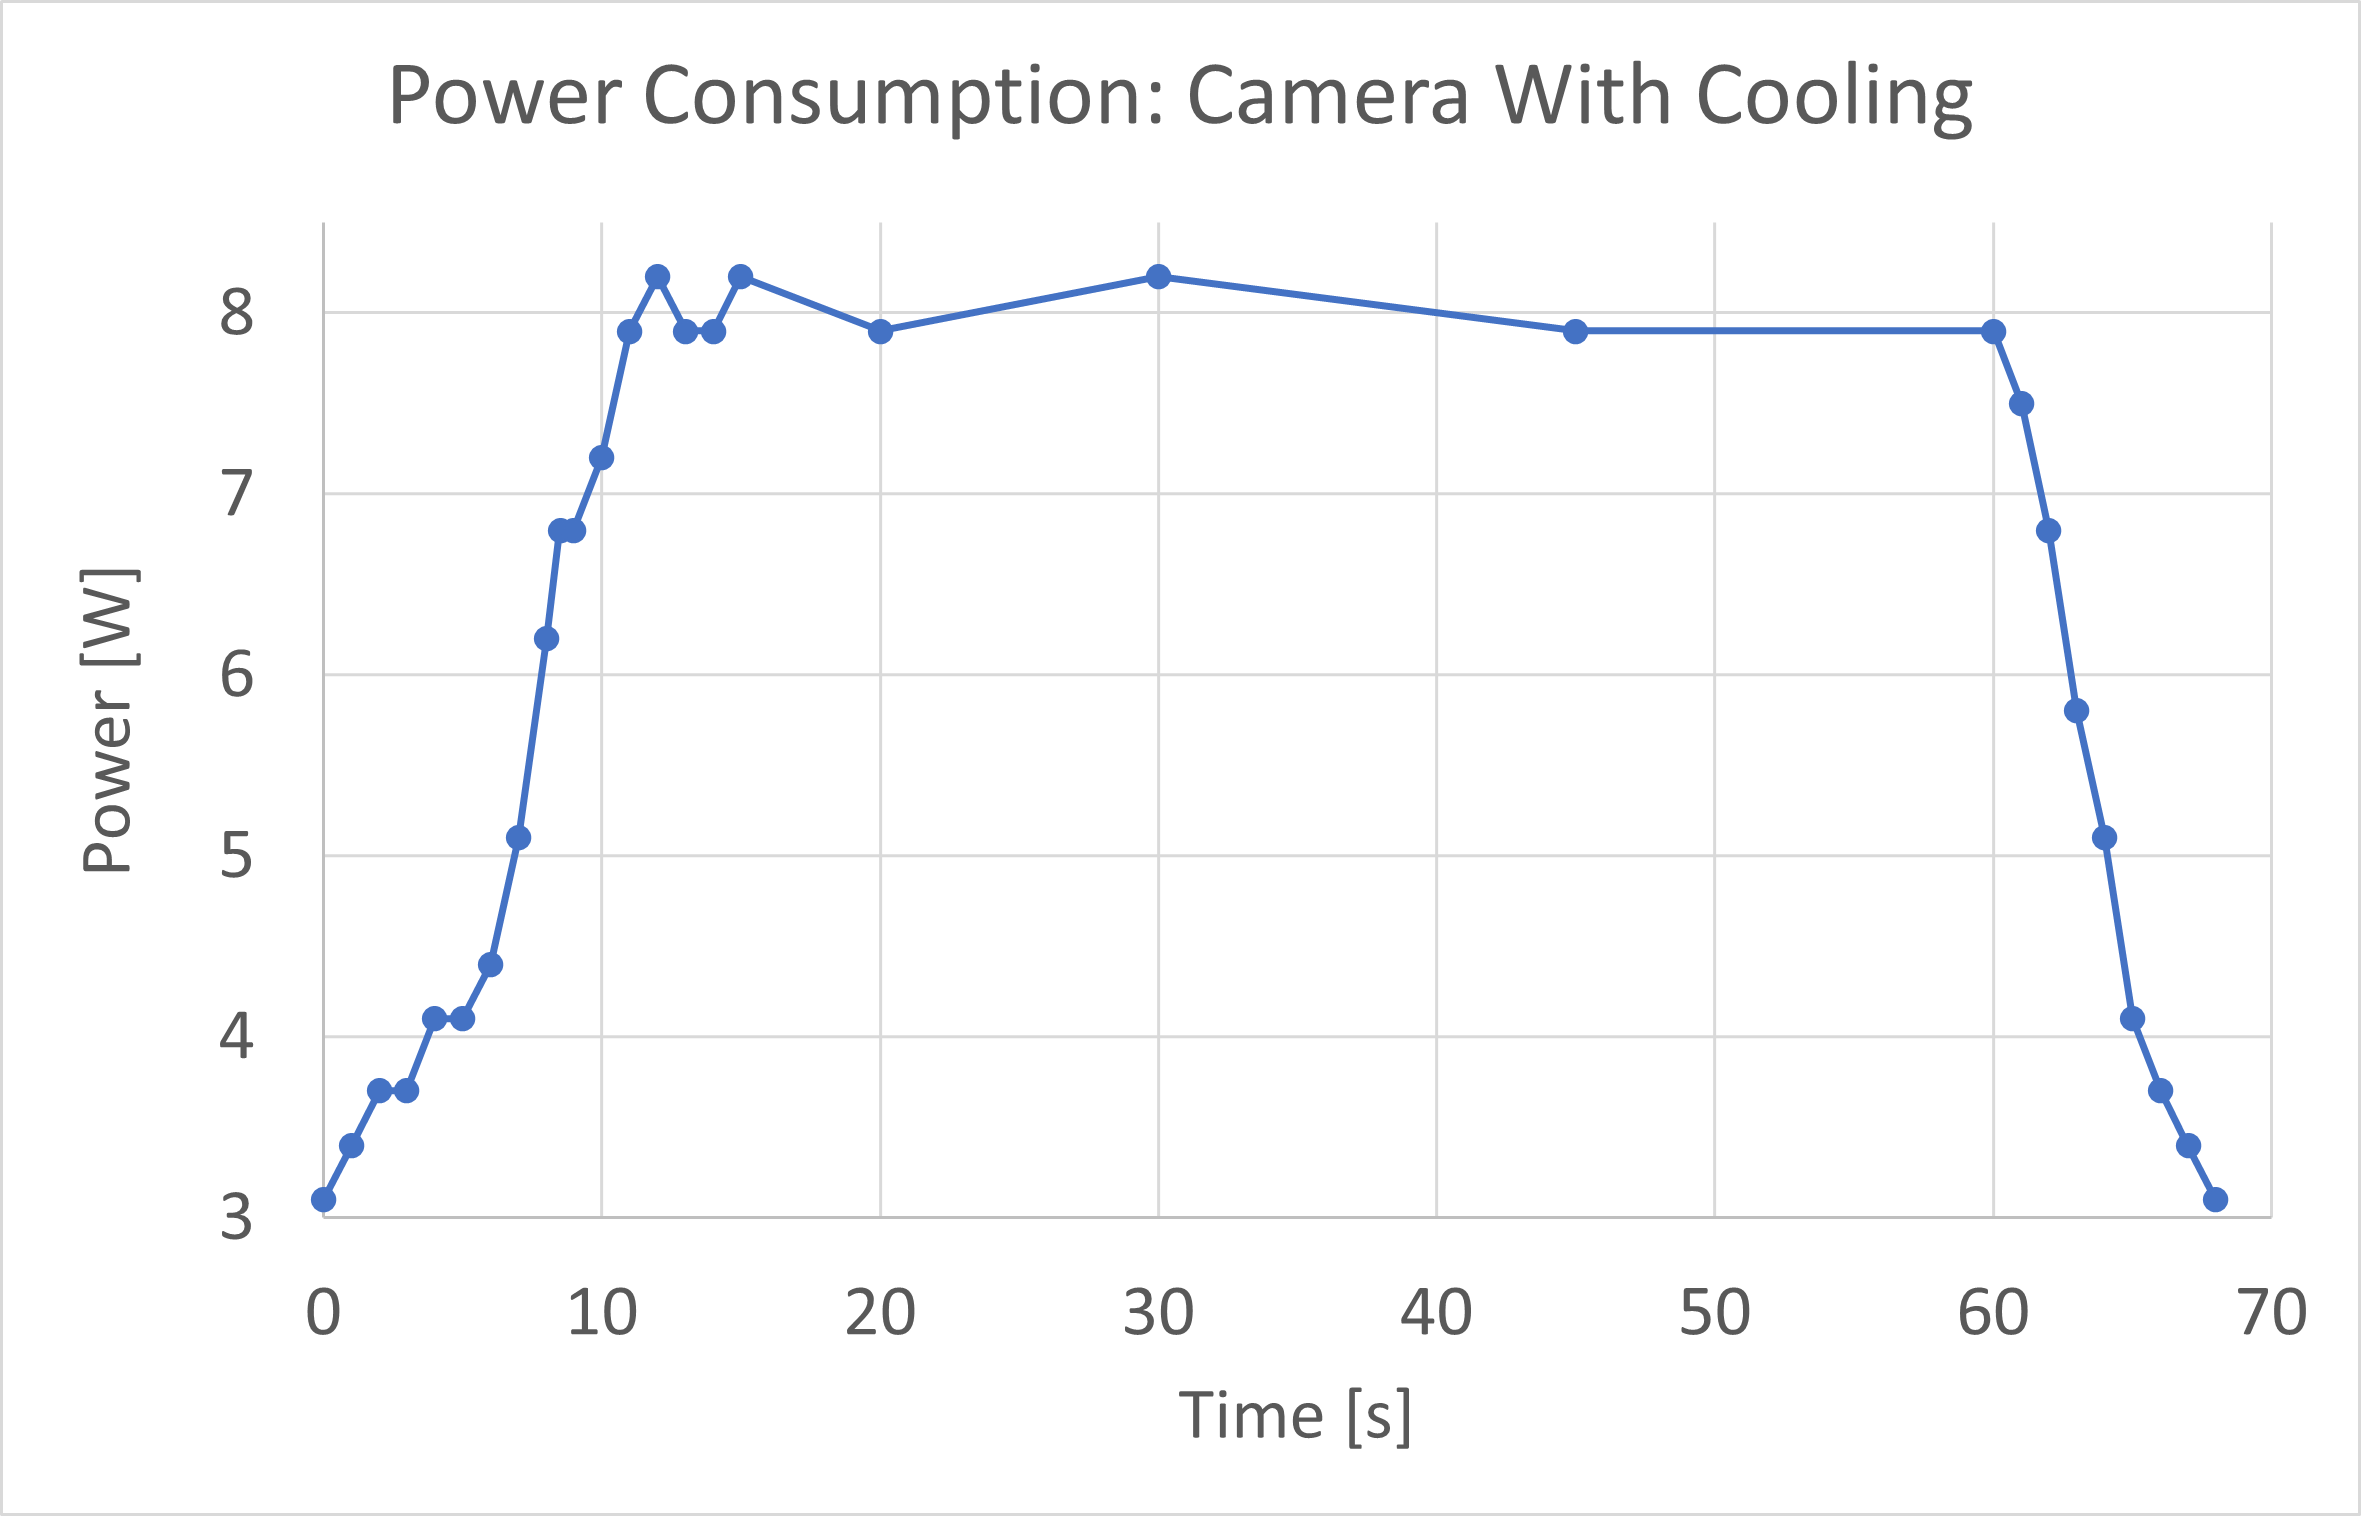
\includegraphics[width=70mm]{Pi_Pictures/Power_C_C.png}}
\caption{Pi 4: Power cooling is applied.}
\label{fig}
\end{figure}

When no cooling is applied, the power drawn is initially high but gradually decreases over time before stabilizing at 6.5W.

\begin{figure}[htbp]
\centerline{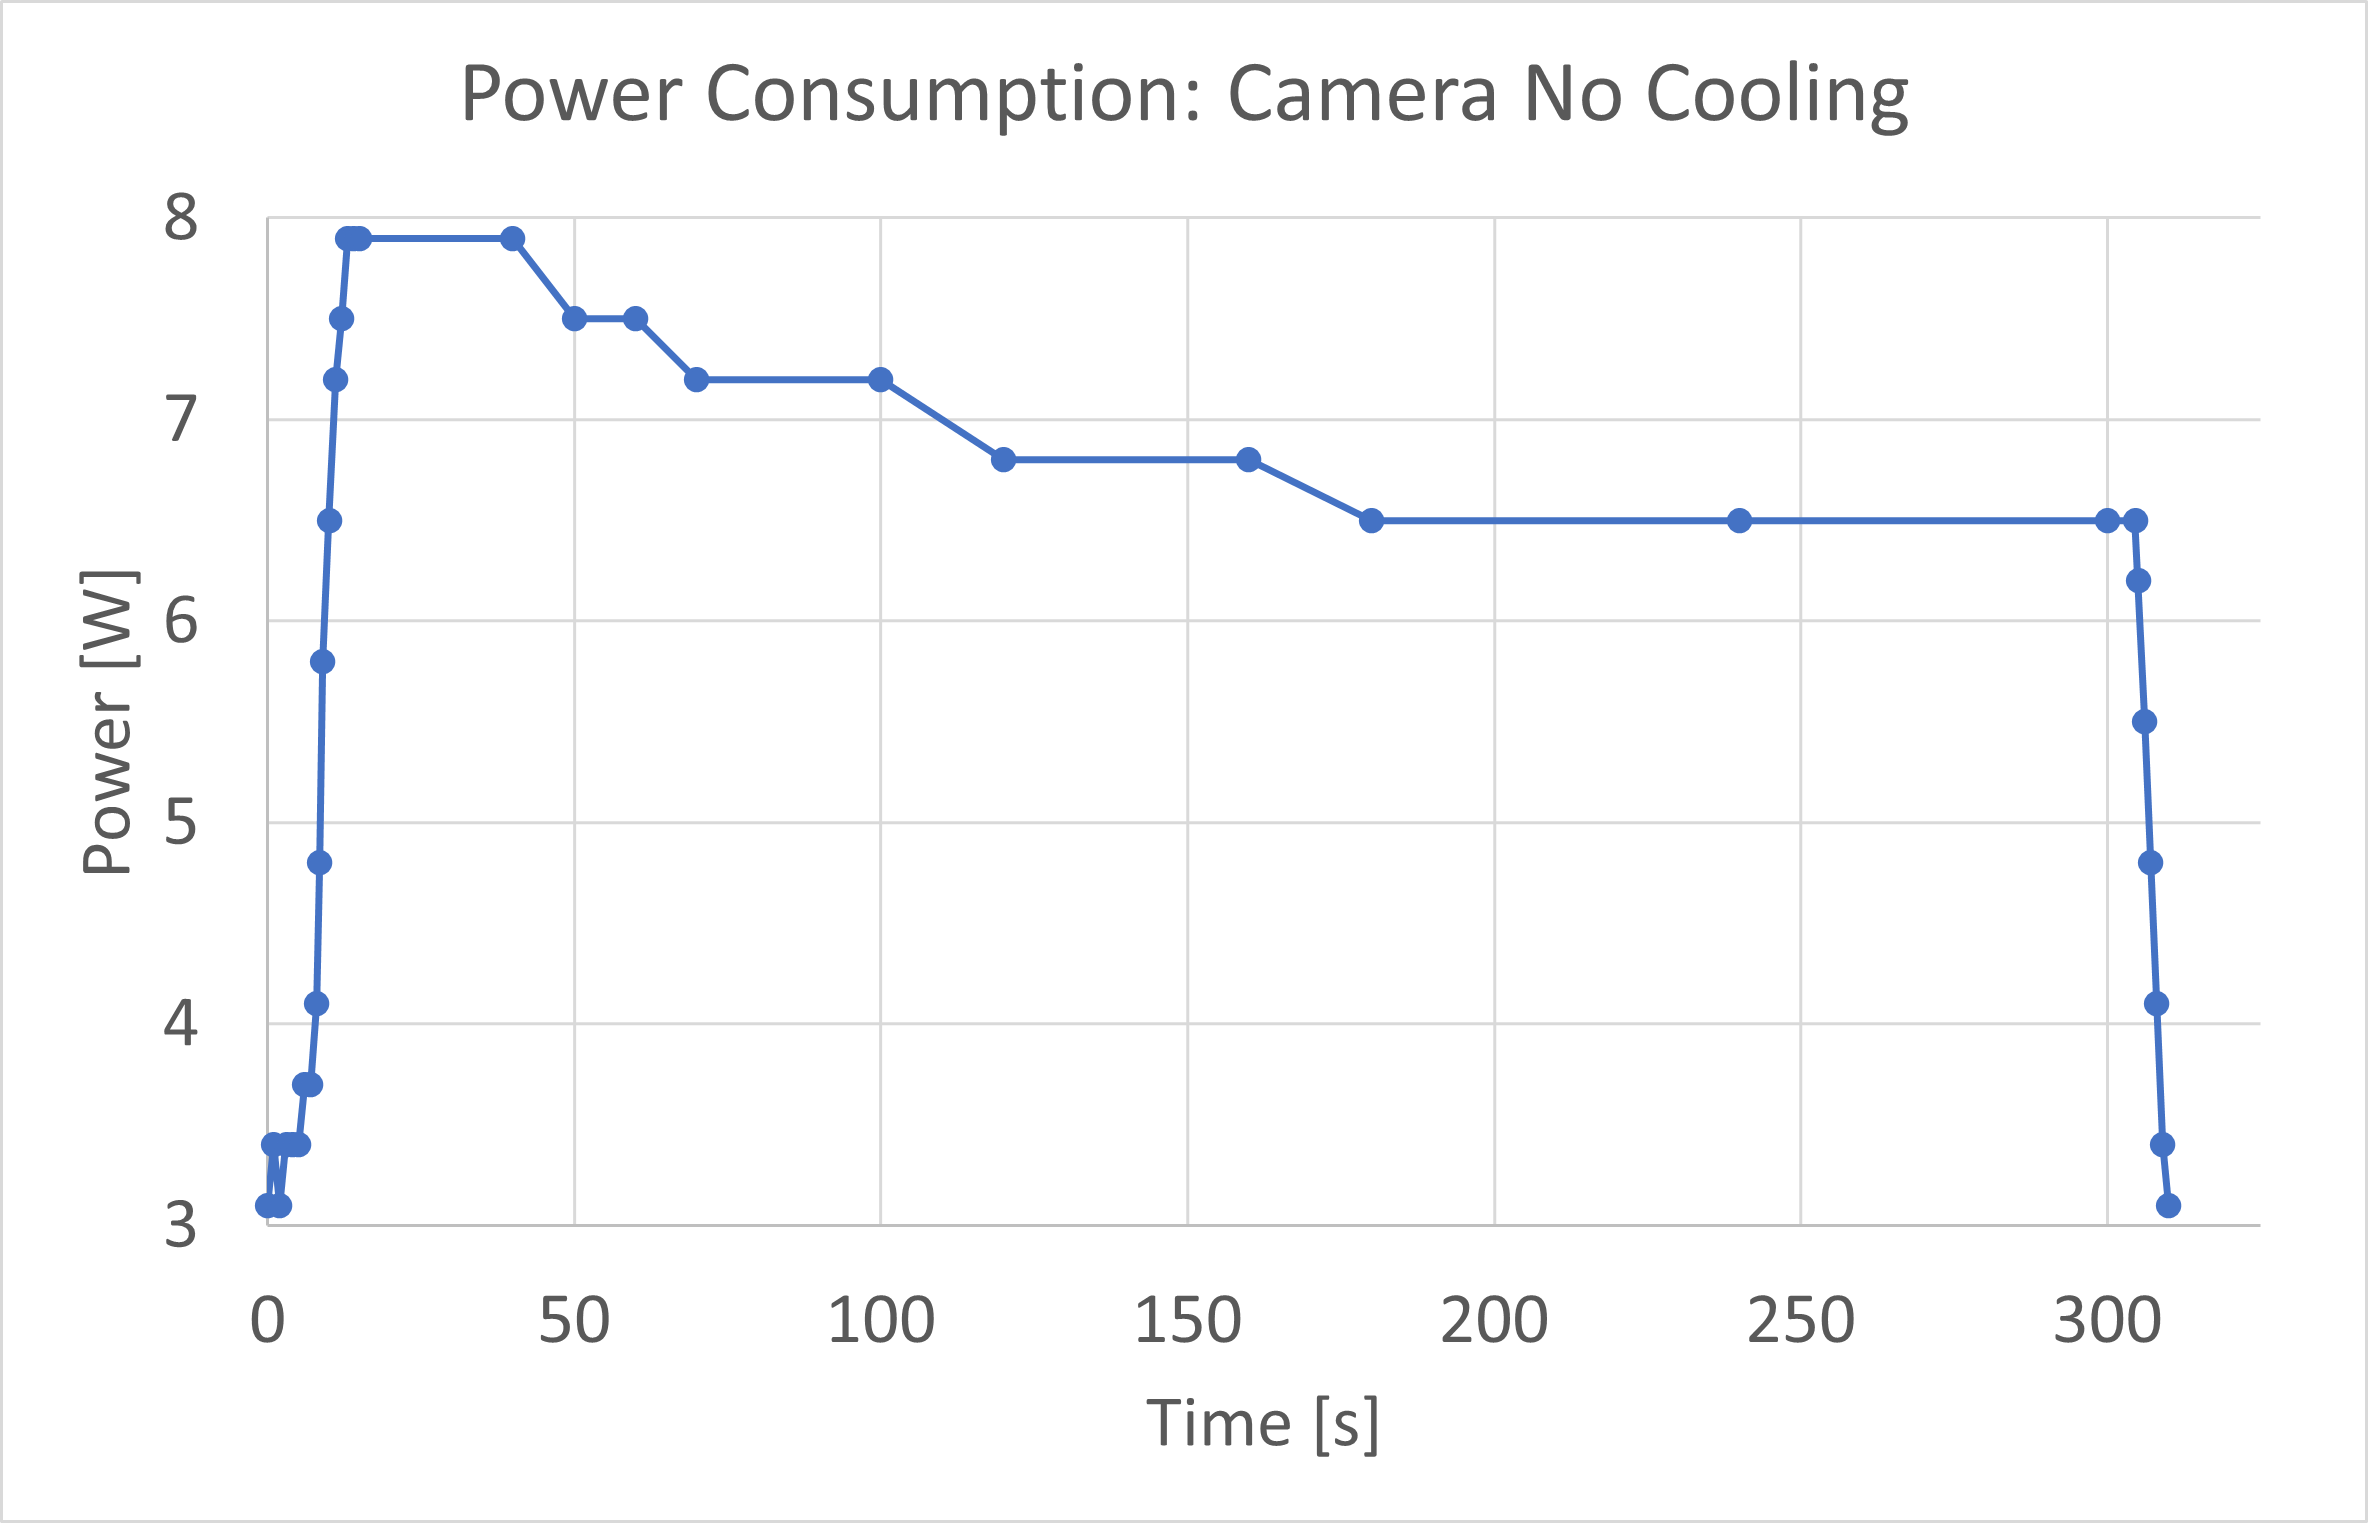
\includegraphics[width=70mm]{Pi_Pictures/Power_C_NC.png}}
\caption{Pi 4: Power when no cooling is applied.}
\label{fig}
\end{figure}

\subsection{YOLOv5: Evaluation}
From our results, the best performance is when images are retrieved from the external SD card. However, many systems require a live camera feed and identify objects using that data.

When the system is cooled, the required power increases but with improvements in performance and power stability. Without cooling, the power requirements are lower, but this comes at the cost of degrading performance and inconsistent power consumption.

Overall, the YOLOv5 algorithm performs poorly on the Raspberry Pi 4. The Pi 4 does not have the hardware required to execute the algorithm with the performance necessary for most practical applications. As a result, a less computationally intensive algorithm is necessary for object detection applications using a Raspberry Pi.

\section{Object Detection on Microcontrollers}
Microcontrollers (MCUs or also known as micros) are simple processors that perform only one task, it can be a simple task like listening to sensors or detecting objects on images [15].

Many limitations exist with using MCUs; for instance, MCUs are limited in memory. A microcontroller typically contains anywhere from hundreds and thousands of bytes [14], limiting the micro's ability to perform a simple task. An additional constraint for MCUs is power, microcontrollers are low-powered and therefore can not handle high-power devices or output high wattage [12]. 

Following the constraints, microcontrollers are limited in the ability to do machine learning (ML) due to the complexity of the process. ML is defined as computer systems that are able to learn and adapt without any clear instructions but simply by following algorithms and models to analyze and draw inferences from data patterns [13]. Machine Learning is not possible on micros because of complex requirements that are necessary from the models. However, ML on microcontrollers is feasible through other possible solutions. 

\subsection{TensorFlow Lite and Microcontroller}
The microcontroller tested was the ESP32. For this part, Raspberry Pi, ESP32 microcontroller, and ESP32 Cam were wired and connected together to perform object detection. This process is only possible if TensorFlow Lite is detecting objects because machine learning can not be done on the microcontroller directly. TensorFlow Lite analyzes the images from the microcontroller and completes the object detection. This idea is different and unique because it allows for object detection to be completed on a tiny device with such a complex build and many limitations. 

\subsection{YOLO and Microcontroller}
An alternative to using the YOLOv5 algorithm was to stream the data from the ESP32 micro and the ESP32 cam to a device that could run YOLOv5. For this section, a laptop would run the YOLOv5 algorithm as it receives the feed from the cam and micro in order to do the object detection and machine learning similar to using TensorFlow. 

\subsection{Results on the Microcontroller}

\begin{figure}[htbp]
\centerline{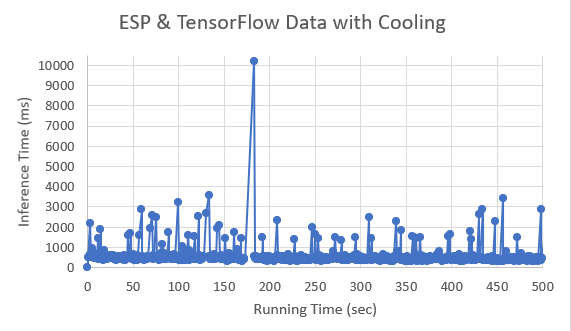
\includegraphics[width=70mm]{Micro/ESP & TensorFlow w cooling.png}}
\caption{Inference time of ESP32 and TensorFlow with cooling.}
\label{fig}
\end{figure}
\begin{figure}[htbp]
\centerline{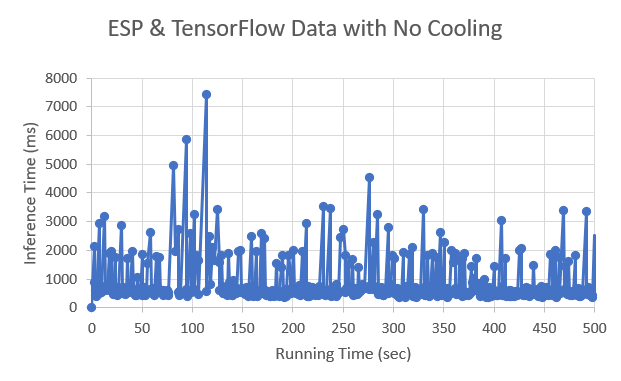
\includegraphics[width=70mm]{Micro/ESP & TensorFlow w no cooling.png}}
\caption{Inference time of ESP32 and TensorFlow with no cooling.}
\label{fig}
\end{figure}

For the ESP32 and TensorFlow, the average FPS rate is 1.28 and the average inference time is 783.43 ms with no cooling. On the other hand, with cooling applied the average FPS rate is 1.90 and the average inference time is 525.67 ms. When cooling is applied to the ESP32 and TensorFlow, the performance time seems to be slower than when no cooling is applied. As seen in the graphs, many spikes occur as a result of instability. The instability is a result of the network latency that occurs due to the Wi-Fi connection. 

\begin{figure}[htbp]
\centerline{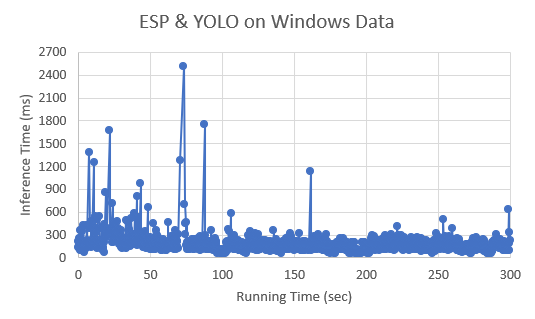
\includegraphics[width=70mm]{Micro/ESP & YOLO on Windows.png}}
\caption{Inference time of ESP32 and YOLO on Windows.}
\label{fig}
\end{figure}

Finally, the analysis for YOLO and Windows has an average FPS rate of 6.04 and the inference time is 165.61 ms. Similar to the ESP32 microcontroller and TensorFlow graphs, this graph contains sudden spikes because of the unstable network. 

For power consumption, the ESP32 micro and the ESP32Cam are negligible. However, when the microcontroller and the camera are connected together with the Raspberry Pi, the power used increases by 0.7W. While idle the Raspberry Pi has a measured power usage of 2.7W, but when connected to the microcontroller, the power increases to 3.4W.

\section{Conclusion}
Object detection algorithms such as YOLOv5 are incredibly powerful when applied to problems requiring computer vision, but are computationally intensive. Modern desktop PCs have the capabilities to process frames and perform inferences fast enough to be useful in many applications. However, if we wish to use object detection on smaller devices or in embedded systems, computational resources and power constraints must be accounted for. If object detection were to be implemented on a microprocessor like a Raspberry Pi, an algorithm like YOLOv5 underperforms, but a less intensive algorithm, like TensorFlow Lite, can run with much greater success. Running YOLOv5 on a microcontroller is infeasible for many of the common microcontrollers on the market, but there are frameworks for running some algorithms like TensorFlow Lite. If an algorithm like YOLOv5 is used with a microcontroller, it is possible to stream the video feed from the microcontroller, process it on another machine, and have the microcontroller respond accordingly. However, this method accrues additional costs and forces internet constraints that bottleneck the overall system. Despite this, it is feasible to process the feed from the ESP32CAM and achieve results in an acceptable time frame despite the bottlenecks of the internet connection.

\section*{Acknowledgment}
We thank Dr.Mohamed El-Hadedy for their guidance and feedback throughout the duration of our studies and work.

\begin{thebibliography}{00}
\bibitem{b1} Ultralytics (2022) YOLOv5 (Version 7.0) [Source Code] https://github.com/ultralytics/yolov5
\bibitem{b2} FreedoomTechWeb (2022) YOLOv5Raspberry Pi 4 [Source Code] https://github.com/freedomwebtech/yolov5raspberry-pi4
\bibitem{b3} TensorFlow (2022) TensorFlow (Version 2.11.0) [Source Code] https://github.com/tensorflow/tensorflow
\bibitem{b4} FreedoomTechWeb (2022) ESP32Cam Object Detection [Source Code] https://github.com/freedomwebtech/esp32camobjectdetection
\bibitem{b5} KUMAN Power Meter KW47
User Manual, KUMAN. Accessed: Sep. 30, 2022. [Online]. Available: https://manuals.plus/kuman/kw47-power-meter-manual
\bibitem{b6} Lauren Hinkel  |  MIT-IBM Watson AI Lab, “Tiny Machine Learning Design alleviates a bottleneck in memory usage on internet-of-things devices,” MIT News | Massachusetts Institute of Technology. [Online]. Available: https://news.mit.edu/2021/tiny-machine-learning-design-alleviates-bottleneck-memory-usage-iot-devices-1208. [Accessed: 26-Nov-2022].
\bibitem{b7} M. Stewart, “Tiny Machine Learning: The next ai revolution,” Medium, 03-Oct-2020. [Online]. Available: https://towardsdatascience.com/tiny-machine-learning-the-next-ai-revolution-495c26463868. [Accessed: 26-Nov-2022]. 
\bibitem{b8} D. Davies, “Yolov5 object detection on windows (step-by-step tutorial),” W\&B, 20-Sep-2021. [Online]. Available: https://wandb.ai/onlineinference/YOLO/reports/YOLOv5-Object-Detection-on-Windows-Step-By-Step-Tutorial---VmlldzoxMDQwNzk4. [Accessed: 26-Nov-2022]. 
\bibitem{b9} J. Cohen, “How to optimize a deep learning model for faster inference?,” Think Autonomous, 19-Oct-2022. [Online]. Available: https://www.thinkautonomous.ai/blog/deep-learning-optimization/. [Accessed: 26-Nov-2022]. 
\bibitem{b10} D. R. Parthasarathi, “Computer Architecture,” Performance Metrics – Computer Architecture, 24-Jul-2018. [Online]. Available: https://www.cs.umd.edu/~meesh/411/CA-online/chapter/performance-metrics/index.html. [Accessed: 26-Nov-2022]. 
\bibitem{b11} Core Temp. [Online]. Available: https://www.alcpu.com/CoreTemp/. [Accessed: 26-Nov-2022]. 
\bibitem{b12} “Advantages and disadvantages of microcontroller,” Polytechnic Hub, Apr. 13, 2017. https://www.polytechnichub.com/advantages-disadvantages-microcontroller/ [Accessed Nov. 27, 2022].
\bibitem{b13} IBM Cloud Education, “What is Machine Learning?,” IBM, Jul. 15, 2020. https://www.ibm.com/cloud/learn/machine-learning [Accessed Nov. 27, 2022].
\bibitem{b14} M. Lab, “Microcontroller Memory Organization and Types - Explained with Memory Segments,” Microcontrollers Lab, Aug. 15, 2020. https://microcontrollerslab.com/microcontroller-memory-organization-types-memory-segments/ [Accessed Nov. 27, 2022].
\bibitem{b15} “Microcontrollers: The Basics – ITP Physical Computing,” Nyu.edu, 2021. https://itp.nyu.edu/physcomp/lessons/microcontrollers-the-basics/.
\end{thebibliography}
\vspace{12pt}

\end{document}
